% manuscript produces a one-column, double-spaced document:
%\documentclass[12pt,preprint]{aastex}
\documentclass[twocolumn]{aastex61}
%\documentclass[iop]{emulateapj}

% preprint2 produces a double-column, single-spaced document:
%\documentclass[preprint2]{aastex}

%Packages
%\usepackage[colorlinks=true,linkcolor=blue,citecolor=blue]{hyperref}

\usepackage{natbib}
\usepackage[caption=false]{subfig}
\usepackage{amsmath,amssymb}
\newcommand{\vdag}{(v)^\dagger}
\newcommand{\degree}{$^\circ$}
\newcommand{\vtan}{$V_{tan}$}
\newcommand{\kms}{km~s$^{-1}$}
\newcommand{\msun}{M$_{\sun}$}
\newcommand{\rjup}{R$_{Jup}$}
\newcommand{\ldl}{$\lambda/{\Delta}{\lambda}$}
\newcommand{\lsun}{L$_{\sun}$}
\newcommand{\lbol}{$\log_{10}{L_{bol}/L_{\sun}}$}
\newcommand{\teff}{T$_{eff}$}
\newcommand{\logg}{$\log{g}$}
\newcommand{\fsed}{$f_{sed}$}
\newcommand{\kzz}{$K_{zz}$}
\newcommand{\meth}{CH$_4$}
\newcommand{\wat}{H$_2$O}
\newcommand{\sha}{KIC 1255 b}
\newcommand{\shStar}{KIC 1255}

%\slugcomment{To be submitted to MNRAS}


\shorttitle{KIC 12557548 b Long Term Followup}
\shortauthors{Schlawin et al.}


\begin{document}


\title{Long Term Monitoring of the Disintegrating Planet Candidate KIC 12557548 b}

%% Use \author, \affil, and the \and command to format
%% author and affiliation information.
%% Note that \email has replaced the old \authoremail command
%% from AASTeX v4.0. You can use \email to mark an email address
%% anywhere in the paper, not just in the front matter.
%% As in the title, use \\ to force line breaks.

\correspondingauthor{E. Schlawin}
\email{eas342@email.arizona.edu}

\author{E. Schlawin}
\affiliation{Steward Observatory, Tucson AZ 85721}

\author{Betsy Green?}
\affiliation{Steward Observatory, Tucson AZ 85721}

\author{J. Teske?}
\affiliation{Carnegie Observatories, 813 Santa Barbara Street, Pasadena, CA 91101, USA}

\author{S. Rappaport?}
\affiliation{MIT}

\author{R. van Lieshout?}
\affiliation{Institute of Astronomy - University of Cambridge}

\begin{abstract}
KIC 12557548 b is one of several disintegrating planet candidates which lose mass in the form of dust particles escaping their surface. Photometric monitoring of KIC 12557548 b originally showed evidence for a slowdown of integration activity in 2013 and 2014. Here, we report 2016 measurements that are consistent with photometry from the Kepler spacecraft in 2009-2013.
We also examine the system with high resolution spectroscopy and discuss the parameters of the host star.
\end{abstract}


\keywords{stars: atmospheres -- stars: individual (\objectname{KIC 12557548}) -- stars: variables: general}

\section{Introduction}
\citet{rappaport} first reported the discovery of a highly unusual stellar system in the Kepler field.
KIC 12557548's (hereafter \shStar's) light curve exhibits periodic flux dips with a period of 0.653 days.
Surprisingly, the flux dips are neither symmetric in shape nor constant in amplitude, varying from $\sim$ 0\% to $\sim$ 1.2\%.
The amplitudes of the flux dips are highly stochastic and unpredictable from one event to the next 0.653 days later.
This indicates the creation and clearing of material that can cover up to 1\% of the star in $\lesssim$ 1 day timescales.
These unusual light curve behaviors are best explained as dust extinction from material that is escaping a rocky planet (KIC 12557548 b, hereafter \sha) in a short period orbit.
The \shStar\ system has the exciting possibility of being an opportunity to study a planet that has been peeled away layer by layer to reveal an interior core.

The discovery of K2-22b \citep{sanchis-ojedak2-22}, WD 1145+017 \citep{vanderburg2015wdDisintegrating}, KOI 2700 \citep{rappaport2014KOI2700} showed that other systems have similar light curves and that other disintegrating planet systems may be useful laboratories for understanding disintegrating planets.
Multi-wavelength light curve measurements show that the dust particles can have wavelength-dependent transmission, as predicted from sub-micron dust particles \citep{bochinski2015evolving,sanchis-ojedak2-22}.

Furthermore, there are perplexing systems that also display stochastic transit behavior but for which there are still no agreed-upon explanations: KIC 8462852 (ie. Boyajian's star) \citep{boyajian846}, RIK-210 \citep{david2017rik210} and PTFO 8-8695 \citep{vanEyken2012ptfTTauri}.
KIC 8462852 may be a family of comets from one or more parent bodies that recently were broken apart.
RIK-210 and PTFO 8-8695 are both in young systems ($\lesssim$ 10 and $\lesssim$3 Myr respectively) so they may are proto-planet candidates.
RIK-210 may have accreting material that causes variable extinction while PTFO 8-8695's orbit may be precessing and causing variations in transit depth depending on its longitude.

The underlying planet candidate \sha\ has not been detected directly, but several observational constraints have placed upper limits on its size and mass.
High precision radial velocity measurements of the host star put an upper limit on the reflex motion due to the planet and constrains the mass to be $\lesssim 1.2 M_{\mathrm Jup}$ \citep{croll2014}.
There is no detection of secondary eclipses of \sha\ with a 3$\sigma$ upper limit of $5 \times 10^{-5}$ in the Kepler bandpass, which means that for an albedo of 0.5, the radius of the planet must be smaller than 4600 km \citep{vanWerkhoven2014}.
The timescale of the variability of the transits gives a mass lot rate of order $\sim M_\oplus/Gyr$, which would indicate a present-day mass of 0.014 $M_\oplus$ when using a radiative-hydrodynamic wind model \citep{perez-becker}.

The Kepler spacecraft performed near-continuous long cadence photometry for KIC 12557548 during its entire main mission lifetime from 2009 to 2013.
During this time, the transit depths averaged around $\sim$0.6\% but varied stochastically from just one 15.7 hour orbit to the next.
\citet{vanWerkhoven2014} analyzed 15 of the total 17 quarters of data and calculated every transit depth during this period.
There were two intervals near obits 50 and 1950 that showed shallower (0.1\%) than average transit depths for roughly one month.

Subsequently, \citet{schlawin2016kic1255} observed 8 total transits of the system for 4 nights in 2013 and 4 nights in 2014 for the $r'$ band using the MORIS imager \citep{Gulbis2011} on SpeX/IRTF \citep{rayner03}.
\citet{schlawin2016kic1255} found that the transit depths were all weaker than $0.43\%$ and that the probably of this randomly occurring based on random behavior from Kepler statistics was around 0.2\%.
This was evidence that the observations occured during weaker periods (as found in \citet{vanWerkhoven2014}'s 15 Kepler quarter analysis) or that the disintegration activity was falling off with time.
We performed follow-up $R$ band photometry of the \shStar\ system to explore whether the disintegration activity is shutting off with time.
We also analyze high resolution spectroscopy of the system to help resolve some of the different stellar parameters reported in the literature.

\begin{deluxetable}{lr}
\tablecaption{List of observations}\label{tab:photSummary}
\tablewidth{0pt}
\tablehead{
\colhead{Date} &
\colhead{Comment} \\
\colhead{UT} & \\
 }
\startdata
2016-06-10 & Clouds \\
2016-06-12 & Clear \\
2016-06-14 & Clear \\
2016-07-12 & Clear \\
2016-07-14 & Mostly clear \\
2016-07-16 & Clear \\
\enddata
\tablenotetext{}{Summary of observations and conditions in this work.}
\end{deluxetable}

\section{Observations}
We observed \sha\ with the Mont4k imager on the 61-inch Kuiper observatory.
Table \ref{tab:photSummary} shows a summary of our observations and the UT dates.
We obtained photometry for 5 nights with good weather on the \sha\ system.



\subsection{Previous Observations}

In order to understand the long term behavior of the \sha\ system, we summarize the available published photometry in Table \ref{tab:prevObs}
The Kepler mission provided the longest time baseline with near continuous photometry for about 4 years in long cadence ($\sim$30 min) mode.
Following the failure of the reaction wheel, there were a few follow-up ground based observations.
\citet{bochinsky2015evolving} obtained multi-color simultaneous photometry ($u'$, $g'$ and $z'$) to characterize the dust in the system.
The ratio of the $g'$ to $z'$ transit depths indeed deviated from unity, which could be fit with an interstellar dust extinction law.
Overall, \citet{bochinisky2015evolving} observed 5 separate nights spanning the expected transit durations and detect 1 transit $\sim$1\% in $g'$ band, 1 transit $\sim$0.1\% in $g'$ band and 3 upper limits of < 0.03\% for the other nights.

For one of the flux dip events, the $g$ band photometry exhibited a deeper transit depth than the $z'$ band.
The ratio 

\begin{deluxetable*}{lrrrr}
\tablecaption{List of published observations}\label{tab:prevObs}
\tablewidth{0pt}
\tablehead{
\colhead{Date Start} &
\colhead{Date End} &
\colhead{Observatory} &
\colhead{Filter} &
\colhead{Reference(s)} \\
UT & UT & & & \\
 }
\startdata
2009-05-13 & 2013-05-11 & Kepler & Open CCD & \citet{borucki2010} \\
2013-07-14 & 2013-07-31 & William Herchel & $u'$, $g'$, $z'$/$i'$ & \citet{bochinski2015evolving} \\
2013-08-13 & 2013-09-03 & IRTF & $r'$, NIR spectroscopy & \citet{schlawin2016kic1255} \\
2014-08-14 & 2013-09-04 & IRTF & $r'$, NIR spectroscopy & \citet{schlawin2016kic1255} \\
2016-06-12 & 2016-06-12 & Kuiper & Harris R & This Work \\
2016-07-12 & 2016-07-16 & Kuiper & Harris R & This Work \\
\enddata
\tablenotetext{}{Summary of published photometric observations of \sha.}
\end{deluxetable*}

\subsection{Photometric Pipeline}

For the photometric reduction, we used the \texttt{ccdproc} package to generate master flat field and bias files.
I combined with an average with a low threshold of 2$\sigma$ and a high threshold of 5$\sigma$.

\begin{figure}
\begin{centering}
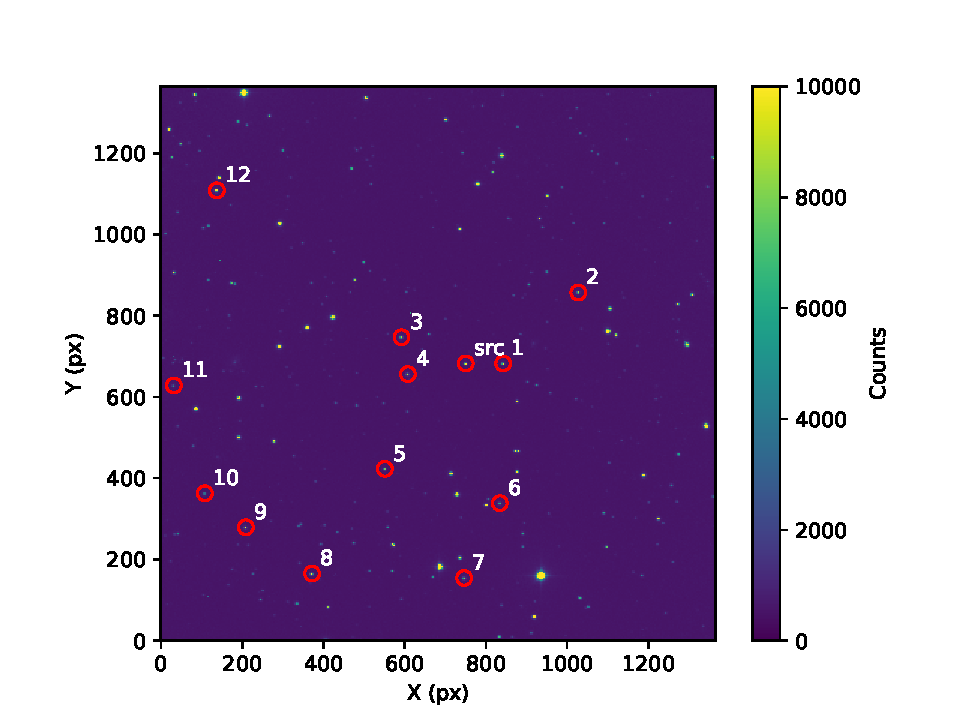
\includegraphics[width=0.5\textwidth]{images/ut2016_07_14_clouds/figure_index_152.pdf}
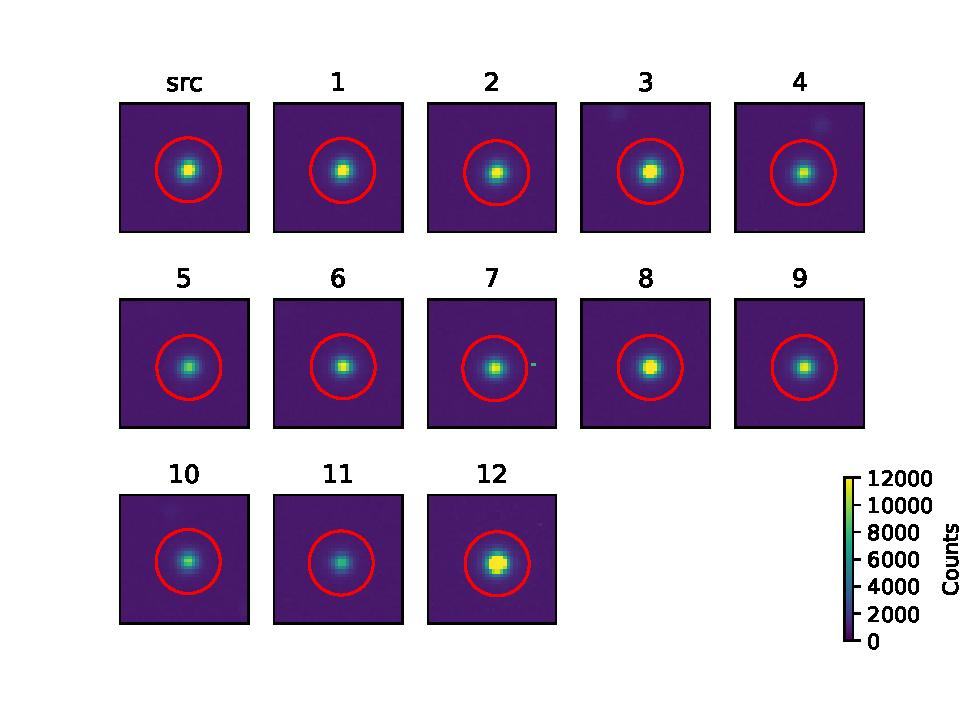
\includegraphics[width=0.5\textwidth]{images/stamps_kic1255_UT2016_07_14.pdf}
\caption{Target (src) and reference stars (numbered) used on UT 2016-07-14.
The reference stars were chosen to have similar count levels as the source. 
}\label{fig:ut2016-07-14cloudImg}
\end{centering}
\end{figure}

All nights light curves are shown in Figure \ref{fig:allNightallStar}.
These are the same reference stars shown in Figure \ref{fig:ut2016-07-14cloudImg}.
The nights two nights in June, 2016 show greater overall stability than the ones in July, 2016.
I suspect that this can mostly be explained by moisture and clouds (such as the ones that caused huge drops in flux on UT2016-07-14.

\begin{figure*}
\begin{centering}
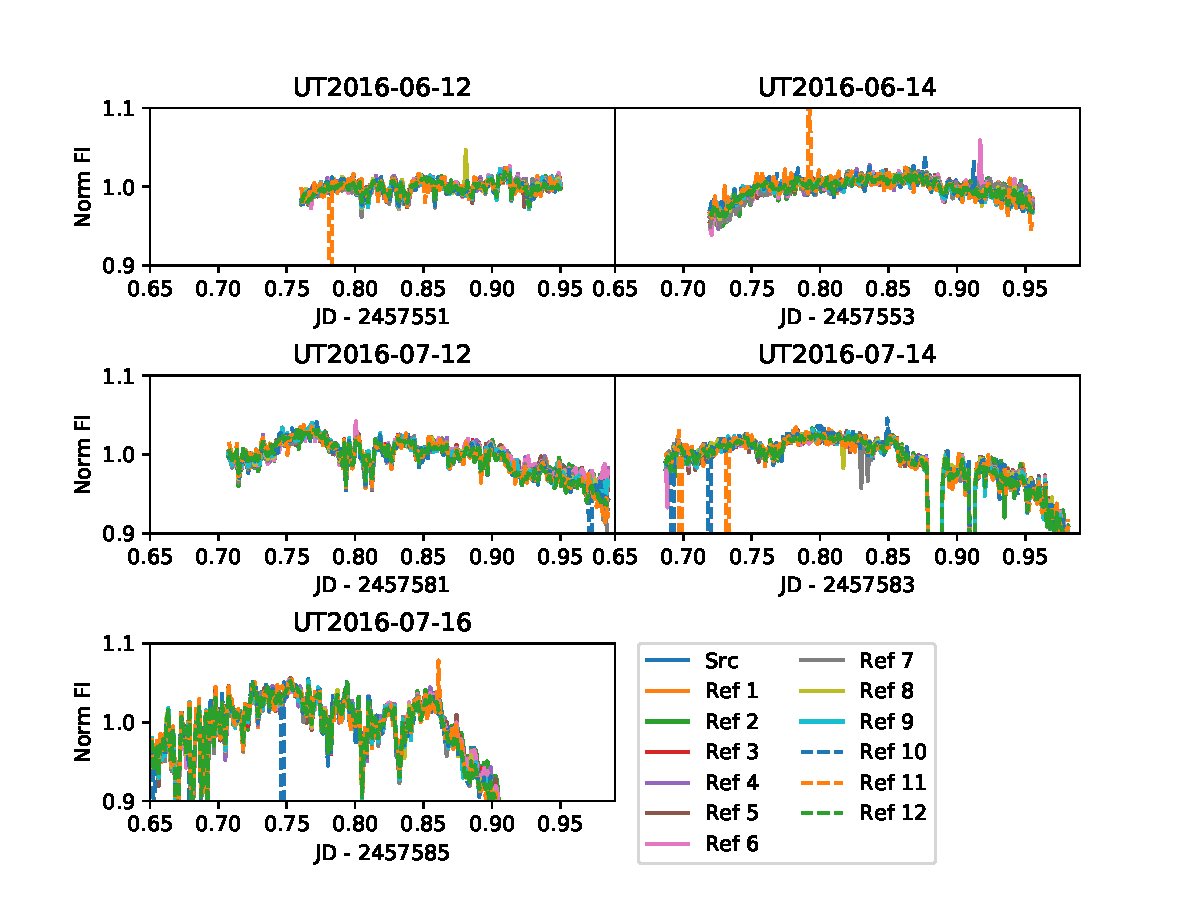
\includegraphics[width=0.9\textwidth]{images/all_kic1255_phot/all_kic1255_allstar.pdf}
\caption{Time series photometry for all stars and all nights nights.
The nights in July appear more strongly affected by cloud/and or seeing variations, whereas the two nights in June are stable to within a few percent.
All source radius, background start and background annulus end parameters were 9, 9 and 12 pixels respectively.}\label{fig:allNightallStar}
\end{centering}
\end{figure*}

Figure \ref{fig:allNightrefCorrect} shows the reference-corrected time series for \shStar\ showing transits.
The expected transit epochs from the ephemeris in \citep{vanWerkhoven2014} are shown for reference.
Typical uncertainties for the Kepler ephemeris are $\sim$ 1 minute at these dates (considering only the uncertainty in period since the transit center is ill-defined).
The ``transit duration'' from Kepler light curves is around 0.05 days, which is consistent with these transit durations.

\begin{figure*}
\begin{centering}
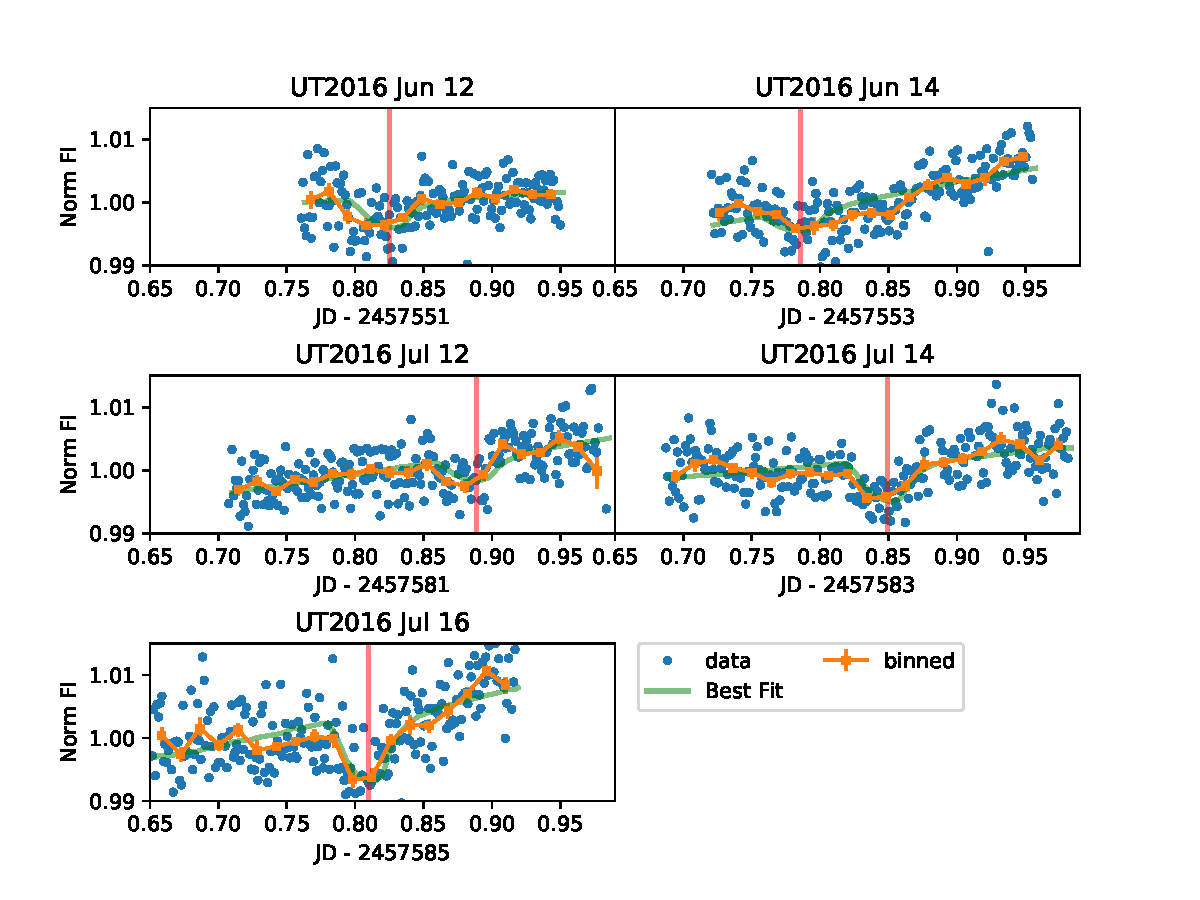
\includegraphics[width=0.9\textwidth]{images/all_kic1255_phot/all_kic1255_refcor.pdf}
\caption{Reference-corrected time series photometry \shStar\ for all nights.
The expected transit epochs from the Kepler-based ephemeris \citep{vanWerkhoven2014} are shown as vertical red bars.
We also show the average Short Cadence Kepler light curves for each of the transit events for comparison with the average.
Transits are clearly visible for all five nights except for UT2016-06-14.}\label{fig:allNightrefCorrect}
\end{centering}
\end{figure*}

\clearpage
\begin{figure}
\begin{centering}
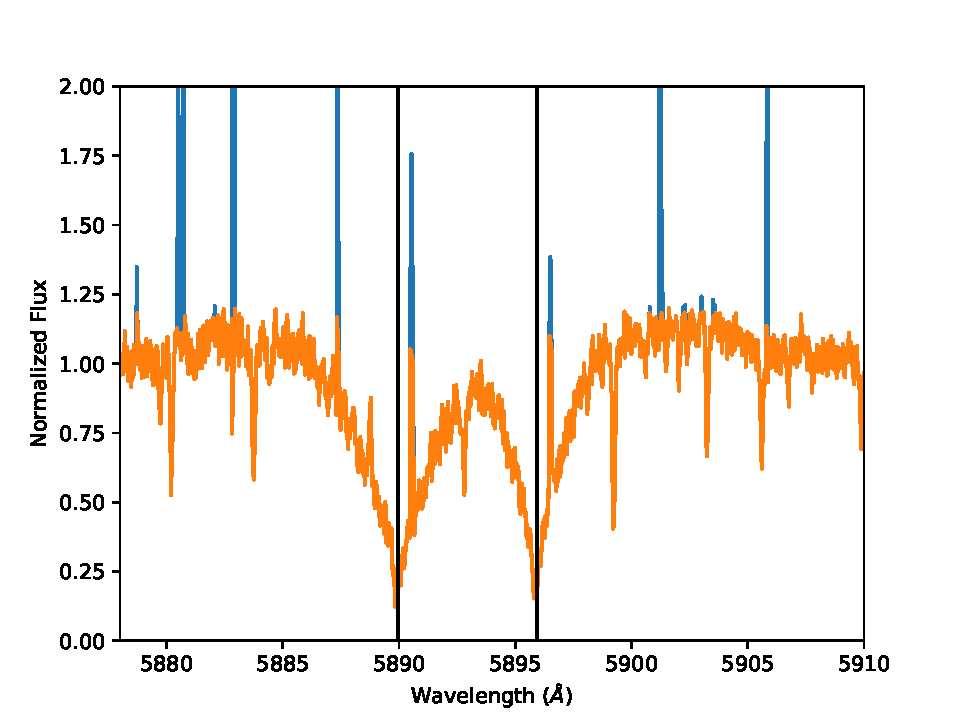
\includegraphics[width=0.45\textwidth]{images/subaru/Na_D_spec_interp.pdf}
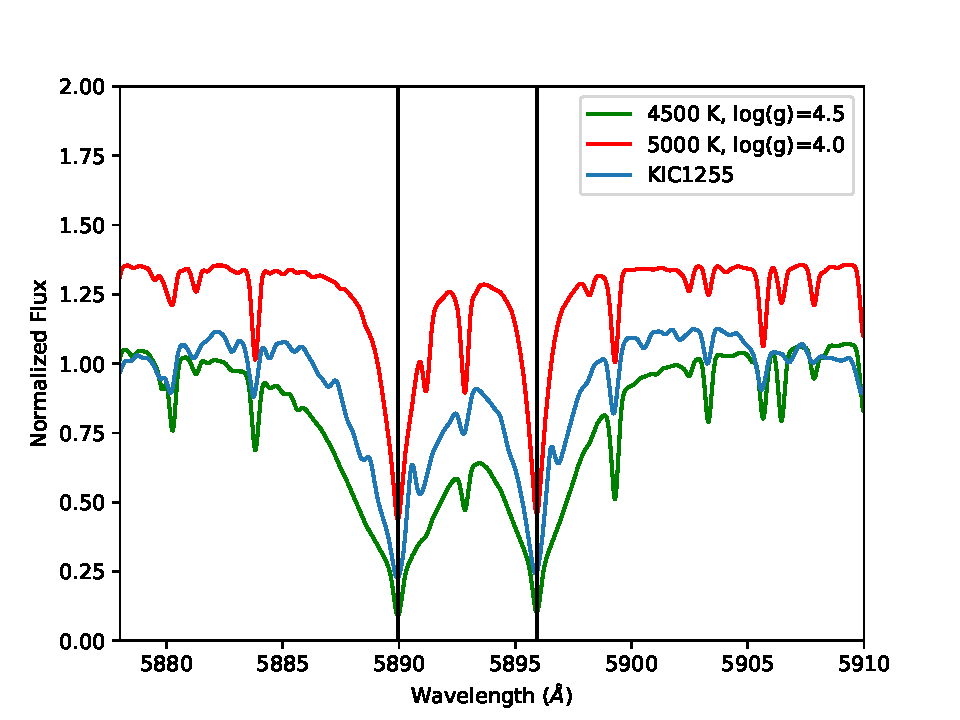
\includegraphics[width=0.45\textwidth]{images/subaru/Na_D_spec.pdf}
\caption{Example spectrum of \shStar\ near the Na D$_1$ and D$_2$ lines (black vertical lines).
There are many bad pixels, which are preliminarily discarded for fluxes above 1.25.
These are not fully removed in the convolved spectrum.}\label{fig:naDlines}
\end{centering}
\end{figure}

\begin{figure}
\begin{centering}
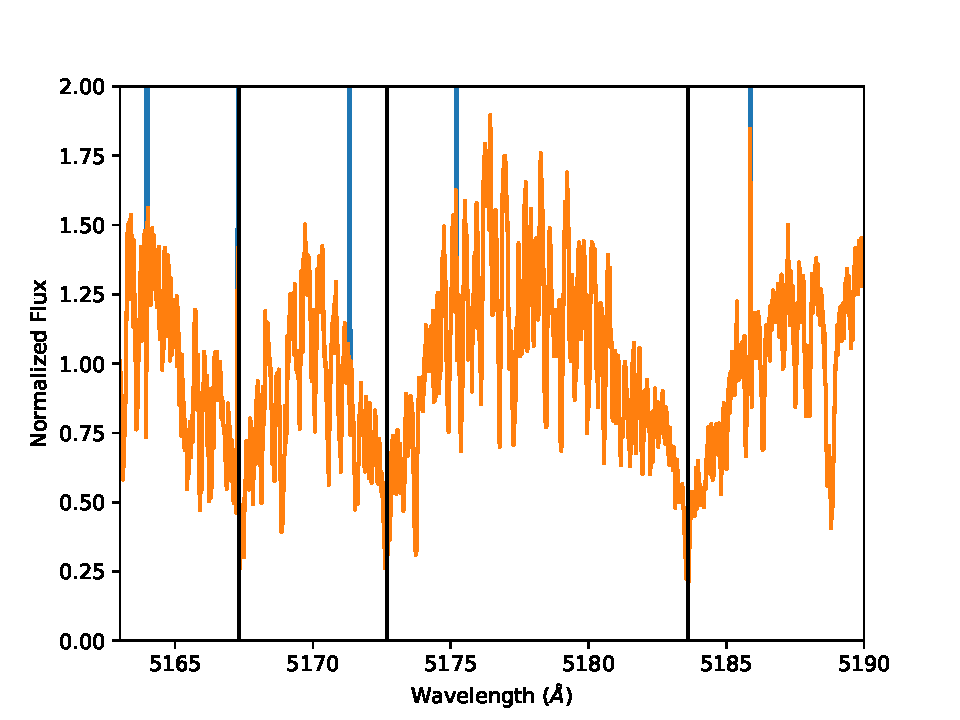
\includegraphics[width=0.45\textwidth]{images/subaru/Mg_triplet_spec_interp.pdf}
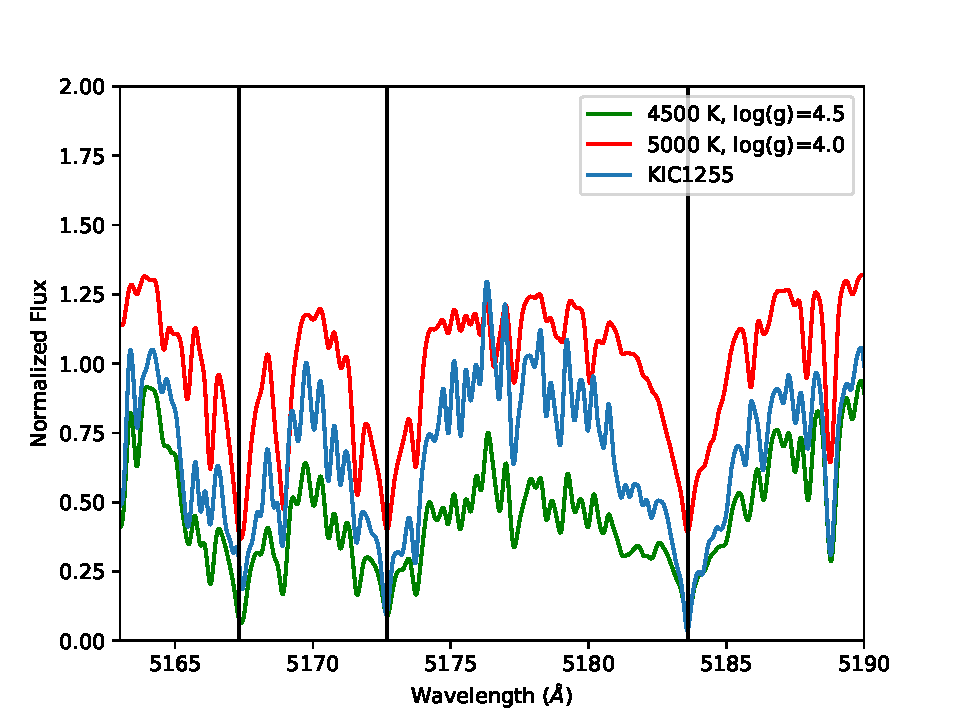
\includegraphics[width=0.45\textwidth]{images/subaru/Mg_triplet_spec.pdf}
\caption{Example spectrum of \shStar\ near the Mg triplet.
{\it Top:} The full resolution original spectrum (blue) is compared to the Mg lines (black) to check wavelength solutions.
The points above a flux of 2.00 are marked as bad pixels and then linear interpolation is performed over these bad pixels to construct a cleaned spectrum (orange).
{\it Bottom} A convolution kernel is applied to the spectrum in order to compare to to HIGHRES models.
The HIGHRES model witha T=4500 K and log(g)=4.5 is a much closer match in terms of line ratios but not the strength of the features.}\label{fig:mgTriplet}
\end{centering}
\end{figure}

\section{Stellar Characterization}
\subsection{Previous Observations}

\begin{deluxetable*}{lcrrr}
\tablecaption{Observational estimates of the stellar parameters of KIC~12557548 from \citet{vanlieshout2016kic1255}}\label{tab:stellObsParams}
\tablewidth{0pt}
\tablehead{
\colhead{Reference} &
\colhead{$ T_{eff,*} $} &
\colhead{$\log(g)$} &
\colhead{Evolutionary Status} &
\colhead{Method} \\
 & (K) & $\log$(cm s$^{-2}$) & & \\
 }
\startdata
  \citet{brown2011kic} & 4400 $\pm$ 200   & 4.6 $\pm$ 0.5    & main-sequence star & photometry \\
  \citet{rappaport}       & 4300 $\pm$ 250    &                            & main-sequence star & low-resolution spectroscopy \\
  \citet{kawahara2013starspots} & 4950 $\pm$ 70 & 3.9 $\pm$ 0.2 & sub-giant          & high-resolution spectroscopy \\
  \citet{huber2014kicprop} & 4550$^{+140}_{-131} $ & 4.622$^{+0.043}_{-0.036} $& main-sequence star & photometry \\
\enddata
\tablenotetext{}{While most of the photometric results show a surface gravity of a main sequence star, the high resolution analysis from \citet{kawahara2013starspots} indicates a gravity consistent with a sub-giant star.}
\end{deluxetable*}


The host star \shStar\ has been characterized by both photometry and spectroscopy.
Table \ref{tab:stellObsParams} shows the summary of observations and analyses compiled in \citet{vanlieshout2016kic1255} for the stellar properties, re-produced here.
In the photometric analysis and low resolution spectroscopy, the spectra are consistent with a 4500 K main sequence K-type star.
High resolution spectra, however, indicate a higher temperature 4900 K lower log(g) sub-giant star \citep{kawahara2013starspots}.
\citet{vanlieshout2016kic1255} analyzed the light curve with a dust model to put constraints on the semi-major axis, which in turn constrains the density of the star when combined with Kepler's third law \citep{seager2003uniqueSolution}.
\citet{vanlieshout2016kic1255} find that the stellar density is only consistent with a main-sequence star with log(g) $\gtrsim 4.4 \log($cm s$^{-2})$.
They suggest an intriguing possibility that the high resolution spectrum of \shStar\ has contamination from dusty debris from the planet and thus appears as a sub-giant star.
If true, this would suggest that high resolution spectra would be valuable tool to study the composition and dynamics of the material escaping \sha.

\subsection{Observations}

We decided to re-visit the high resolution spectrum from \citet{kawahara2013starspots} by downloading the raw data from the Subaru SMOKA database.
We follow the \texttt{iraf} reduction techniques from the instrument manual\footnote{https://www.subarutelescope.org/Observing/Instruments/\\HDS/specana2014.10e.pdf}.
Some modifications to the manual were made, including a more aggressive -50/+50 lower and upper window for bad pixel identification with \texttt{mkbadpx} on the red CCD.
We applied bad pixel masks and bias files to each CCD separately.
Since \shStar\ is smaller than the background flux, we use a spectrum of KOI-678 (Kepler 211) to trace the spectrum and use this trace for \shStar.

\begin{figure}
\begin{centering}
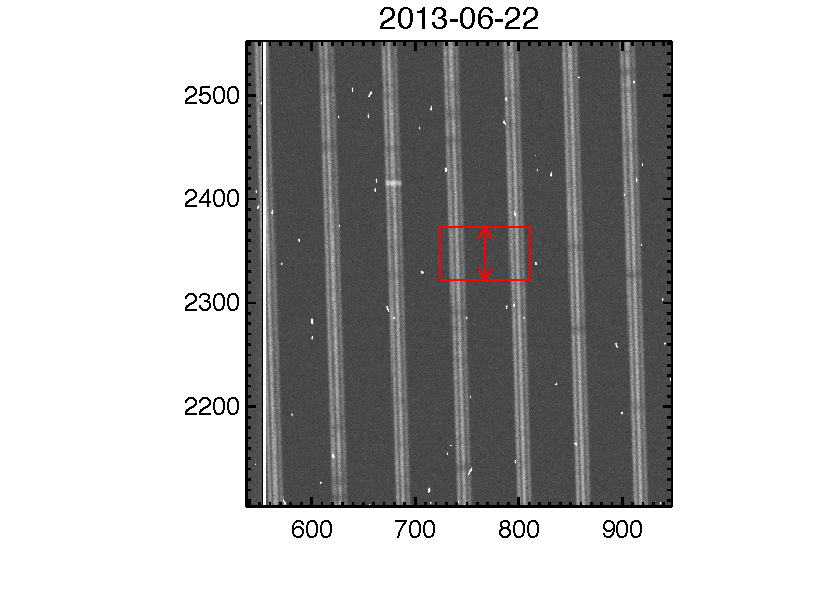
\includegraphics[width=0.4\textwidth]{images/subaru/2013_vs_2015/out_HDSA00094087.pdf}
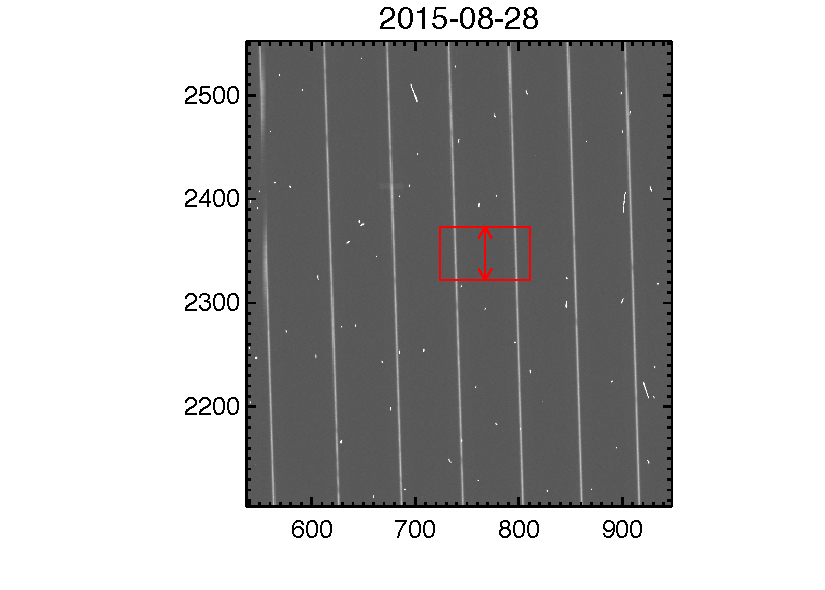
\includegraphics[width=0.4\textwidth]{images/subaru/2013_vs_2015/HDSA00111345.pdf}
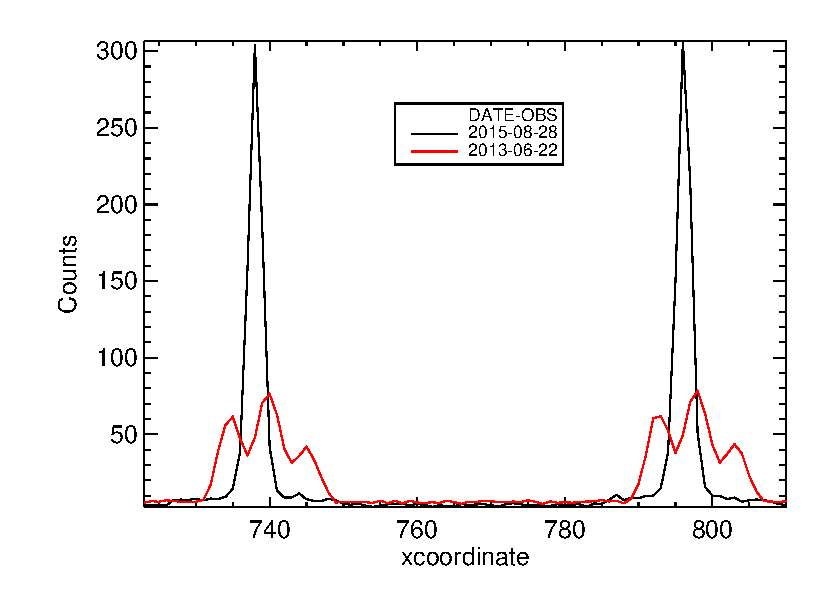
\includegraphics[width=0.45\textwidth]{images/subaru/2013_vs_2015/profile_comparison.pdf}
\caption{Spectra images from 2013 versus 2015. The PSF profile (bottom panel) is much wider in 2013 because an image slicer creates 3 traces for the one star. In 2015, a narrow slit is used instead.}\label{fig:prof2013vs2015}
\end{centering}
\end{figure}

The 2013 HDS data and 2015 HDS data were taken in slightly different modes.
Figure \ref{fig:prof2013vs2015} shows an example blue-chip image from 2013 and 2015.
The 2015 data, with a narrow slit (0.3 $\times$ 3.5 mm) has a sharper PSF and and is easier to trace.
The 2013 data was taken with a wider (2 $\times$ 30 mm) slit and an image slicer, which create 3 parallel traces for \shStar.
A flat field with a narrower (0.3 mm) slit is needed to create a trace for use with the image slicer.
For wavelength identification, a Thorium Argon reference is used.
(Not to self:) The IRAF order 39 appears to be near 6370 $\AA$ to 6450 $\AA$ which is Order 95/Aperture 16 in the Subaru HDS Th-Ar atlas.
The Th-Ar line identification was started with the atlas, rejecting high sigma points and then used to find the rest of the lines automatically.
The final fit was performed with a chebyshev polynomial, 4th order in x direction and 4th order in y direction.
The final rms in this wavelength solution is 0.0021 $\AA$.
After the reference spectrum is used to find a wavelength solution, the spectrum is examined some strong stellar lines, including the Na D$_1$/D$_2$ lines (Figure \ref{fig:naDlines} and the 

\subsection{Comparison to Templates}

The Mg Triplet (Figure \ref{fig:mgTriplet}) is diagnostic of spectral type and may help resolve some of the conflicts in the literature about the gravity of the host star.
\citet{kawahara2013starspots} find a log(g) = 3.9 $\pm$ 0.2, whereas \citet{rappaport} find a log(g)=4.63.
To compare to some HIGHRES models \citep{coelho2014hires}, we first had to convolve the spectrum.
Also, we interpolated over any pixels above a normalized flux of 2.0 in Figure \ref{fig:mgTriplet} (top).
Then, we convolve with a Gaussian kernel with a standard deviation of 6 pixels.

The region near the Mg triplet in Figure \ref{fig:mgTriplet} is a closer match in terms of line ratios to the higher log(g) =4.5 and T=4500 K spectrum from HIGHRES, but not the line strengths.

\begin{figure}[!hbtp]
\begin{centering}
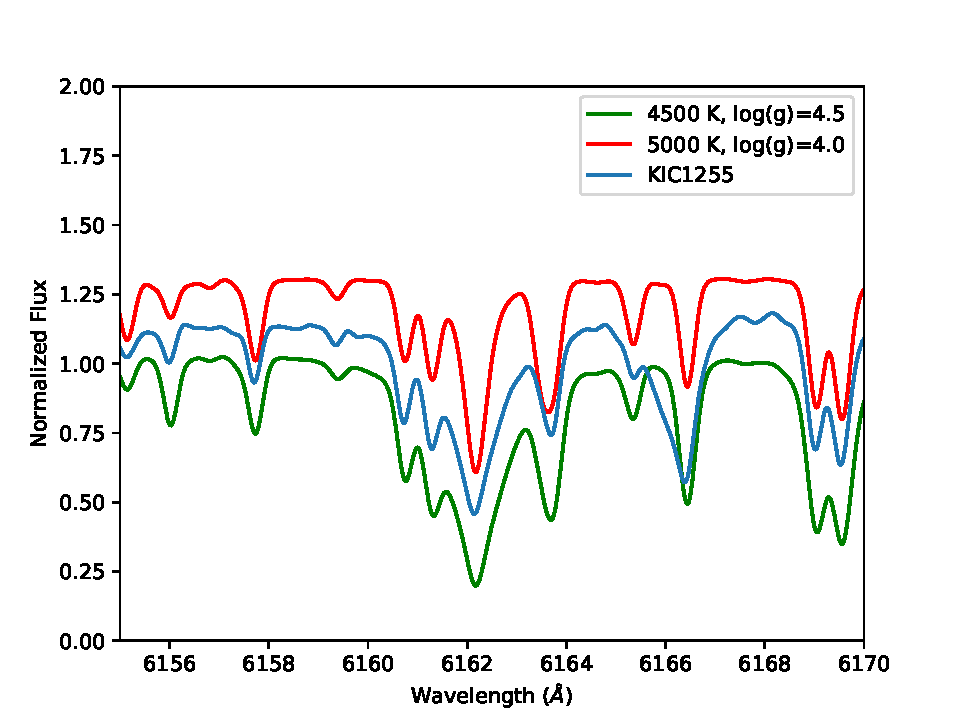
\includegraphics[width=0.45\textwidth]{images/subaru/CaI6162_spec.pdf}
\caption{Example spectrum of \shStar\ near Ca I 6162 $\AA$, another gravity sensitive line.}\label{fig:mgTriplet}
\end{centering}
\end{figure}

\subsection{Comparison to BOSZ}

The BOSZ models \citep{bohlin2017bosz} are calculated up to a resolution of 300,000, so we use these to compare to the measured spectra.
We start by comparing R=100,000 models with the measured spectrum of \shStar\ near the Mg triplet, shown in Figure \ref{fig:mgTriplet}.

\begin{figure}[!hbtp]
\begin{centering}
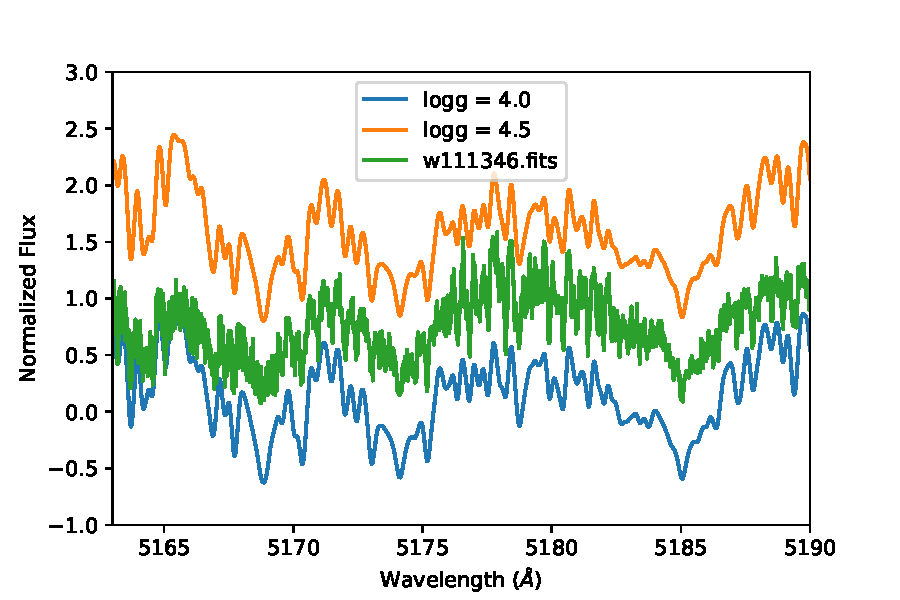
\includegraphics[width=0.45\textwidth]{images/subaru/bosz_mg_triplet.pdf}
\caption{Example spectrum of \shStar\ (reduced by Kento Masuda) near the Mg triplet compared to 4500 K BOSZ models with two different log(g)s.}\label{fig:mgTriplet}
\end{centering}
\end{figure}

\clearpage
\section{Conclusions}\label{sec:conclusions}

\section{Acknowledgements}
Thanks to Alessondra Springman for good resources on core and mantle compositions and the gases that could sublimate off of them.
Thanks to Jonathan Fraine and Rafia Bushra for help with observing at the 61-inch Kuiper telescope on Mt Bigelow.
MCMC fitting makes use of \texttt{emcee} \citep{foreman-mackey2013emcee} and the covariance plot was made with \texttt{corner.py} \citep{foremanCorner}.
Funding for the E Schlawin is provided by NASA Goddard Spaceflight Center.
This research made use of the \texttt{astropy} package \citep{astropy2013}.

%If  used, this work made use of the \texttt{astropy} package \citep{astropy2013}.
%If used, some data was collected from the Open Exoplanet Catalogue \citep{rein2012openExoCat}.

%% In a manner similar to \objectname authors can provide links to dataset
%% hosted at participating data centers via the \dataset{} command.  The
%% second curly bracket argument is printed in the text while the first
%% parentheses argument serves as the valid data set identifier.  Large
%% lists of data set are best provided in a table (see Table 3 for an example).
%% Valid data set identifiers should be obtained from the data center that
%% is currently hosting the data.
%%
%% Note that AASTeX interprets everything between the curly braces in the 
%% macro as regular text, so any special characters, e.g. "#" or "_," must be 
%% preceded by a backslash. Otherwise, you will get a LaTeX error when you 
%% compile your manuscript.  Special characters do not 
%% need to be escaped in the optional, square-bracket argument.



%% In this section, we use  the \subsection command to set off
%% a subsection.  \footnote is used to insert a footnote to the text.

%% Observe the use of the LaTeX \label
%% command after the \subsection to give a symbolic KEY to the
%% subsection for cross-referencing in a \ref command.
%% You can use LaTeX's \ref and \label commands to keep track of
%% cross-references to sections, equations, tables, and figures.
%% That way, if you change the order of any elements, LaTeX will
%% automatically renumber them.

%% This section also includes several of the displayed math environments
%% mentioned in the Author Guide.


%% The equation environment wil produce a numbered display equation.


%% The \notetoeditor{TEXT} command allows the author to communicate
%% information to the copy editor.  This information will appear as a
%% footnote on the printed copy for the manuscript style file.  Nothing will
%% appear on the printed copy if the preprint or
%% preprint2 style files are used.

%% The eqnarray environment produces multi-line display math. The end of
%% each line is marked with a \\. Lines will be numbered unless the \\
%% is preceded by a \nonumber command.
%% Alignment points are marked by ampersands (&). There should be two
%% ampersands (&) per line.

%% Putting eqnarrays or equations inside the mathletters environment groups
%% the enclosed equations by letter. For instance, the eqnarray below, instead
%% of being numbered, say, (4) and (5), would be numbered (4a) and (4b).
%% LaTeX the paper and look at the output to see the results.

%% This section contains more display math examples, including unnumbered
%% equations (displaymath environment). The last paragraph includes some
%% examples of in-line math featuring a couple of the AASTeX symbol macros.

%% The displaymath environment will produce the same sort of equation as
%% the equation environment, except that the equation will not be numbered
%% by LaTeX.
%% If you wish to include an acknowledgments section in your paper,
%% separate it off from the body of the text using the \acknowledgments
%% command.

%% Included in this acknowledgments section are examples of the
%% AASTeX hypertext markup commands. Use \url without the optional [HREF]
%% argument when you want to print the url directly in the text. Otherwise,
%% use either \url or \anchor, with the HREF as the first argument and the
%% text to be printed in the second.

\acknowledgments



%% To help institutions obtain information on the effectiveness of their
%% telescopes, the AAS Journals has created a group of keywords for telescope
%% facilities. A common set of keywords will make these types of searches
%% significantly easier and more accurate. In addition, they will also be
%% useful in linking papers together which utilize the same telescopes
%% within the framework of the National Virtual Observatory.
%% See the AASTeX Web site at http://aastex.aas.org/
%% for information on obtaining the facility keywords.

%% After the acknowledgments section, use the following syntax and the
%% \facility{} macro to list the keywords of facilities used in the research
%% for the paper.  Each keyword will be checked against the master list during
%% copy editing.  Individual instruments or configurations can be provided 
%% in parentheses, after the keyword, but they will not be verified.

%{\it Facilities:} \facility{Nickel}, \facility{HST (STIS)}, \facility{CXO (ASIS)}.

%% Appendix material should be preceded with a single \appendix command.
%% There should be a \section command for each appendix. Mark appendix
%% subsections with the same markup you use in the main body of the paper.

%% Each Appendix (indicated with \section) will be lettered A, B, C, etc.
%% The equation counter will reset when it encounters the \appendix
%% command and will number appendix equations (A1), (A2), etc.

\appendix

\section{Original Light Curves}

%% The reference list follows the main body and any appendices.
%% Use LaTeX's thebibliography environment to mark up your reference list.
%% Note \begin{thebibliography} is followed by an empty set of
%% curly braces.  If you forget this, LaTeX will generate the error
%% "Perhaps a missing \item?".
%%
%% thebibliography produces citations in the text using \bibitem-\cite
%% cross-referencing. Each reference is preceded by a
%% \bibitem command that defines in curly braces the KEY that corresponds
%% to the KEY in the \cite commands (see the first section above).
%% Make sure that you provide a unique KEY for every \bibitem or else the
%% paper will not LaTeX. The square brackets should contain
%% the citation text that LaTeX will insert in
%% place of the \cite commands.

%% We have used macros to produce journal name abbreviations.
%% AASTeX provides a number of these for the more frequently-cited journals.
%% See the Author Guide for a list of them.

%% Note that the style of the \bibitem labels (in []) is slightly
%% different from previous examples.  The natbib system solves a host
%% of citation expression problems, but it is necessary to clearly
%% delimit the year from the author name used in the citation.
%% See the natbib documentation for more details and options.

\bibliographystyle{apj}
\bibliography{ms}

%\clearpage

%% Use the figure environment and \plotone or \plottwo to include
%% figures and captions in your electronic submission.
%% To embed the sample graphics in
%% the file, uncomment the \plotone, \plottwo, and
%% \includegraphics commands
%%
%% If you need a layout that cannot be achieved with \plotone or
%% \plottwo, you can invoke the graphicx package directly with the
%% \includegraphics command or use \plotfiddle. For more information,
%% please see the tutorial on "Using Electronic Art with AASTeX" in the
%% documentation section at the AASTeX Web site, http://aastex.aas.org/
%%
%% The examples below also include sample markup for submission of
%% supplemental electronic materials. As always, be sure to check
%% the instructions to authors for the journal you are submitting to
%% for specific submissions guidelines as they vary from
%% journal to journal.

%% This example uses \plotone to include an EPS file scaled to
%% 80% of its natural size with \epsscale. Its caption
%% has been written to indicate that additional figure parts will be
%% available in the electronic journal.

%\begin{figure}
%\epsscale{.80}
%\plotone{f1.eps}
%\caption{Derived spectra for 3C138 \citep[see][]{heiles03}. Plots for all sources are available
%in the electronic edition of {\it The Astrophysical Journal}.\label{fig1}}
%\end{figure}

%\clearpage

%% Here we use \plottwo to present two versions of the same figure,
%% one in black and white for print the other in RGB color
%% for online presentation. Note that the caption indicates
%% that a color version of the figure will be available online.
%%

%\begin{figure}
%\plottwo{f2.eps}{f2_color.eps}
%\caption{A panel taken from Figure 2 of \citet{rudnick03}. 
%See the electronic edition of the Journal for a color version 
%of this figure.\label{fig2}}
%\end{figure}

%% This figure uses \includegraphics to scale and rotate the still frame
%% for an mpeg animation.

%\begin{figure}
%\includegraphics[angle=90,scale=.50]{f3.eps}
%\caption{Animation still frame taken from \citet{kim03}.
%This figure is also available as an mpeg
%animation in the electronic edition of the
%{\it Astrophysical Journal}.}
%\end{figure}

%% If you are not including electonic art with your submission, you may
%% mark up your captions using the \figcaption command. See the
%% User Guide for details.
%%
%% No more than seven \figcaption commands are allowed per page,
%% so if you have more than seven captions, insert a \clearpage
%% after every seventh one.

%% Tables should be submitted one per page, so put a \clearpage before
%% each one.

%% Two options are available to the author for producing tables:  the
%% deluxetable environment provided by the AASTeX package or the LaTeX
%% table environment.  Use of deluxetable is preferred.
%%

%% Three table samples follow, two marked up in the deluxetable environment,
%% one marked up as a LaTeX table.

%% In this first example, note that the \tabletypesize{}
%% command has been used to reduce the font size of the table.
%% We also use the \rotate command to rotate the table to
%% landscape orientation since it is very wide even at the
%% reduced font size.
%%
%% Note also that the \label command needs to be placed
%% inside the \tablecaption.

%% This table also includes a table comment indicating that the full
%% version will be available in machine-readable format in the electronic
%% edition.

%% If you use the table environment, please indicate horizontal rules using
%% \tableline, not \hline.
%% Do not put multiple tabular environments within a single table.
%% The optional \label should appear inside the \caption command.



%% If the table is more than one page long, the width of the table can vary
%% from page to page when the default \tablewidth is used, as below.  The
%% individual table widths for each page will be written to the log file; a
%% maximum tablewidth for the table can be computed from these values.
%% The \tablewidth argument can then be reset and the file reprocessed, so
%% that the table is of uniform width throughout. Try getting the widths
%% from the log file and changing the \tablewidth parameter to see how
%% adjusting this value affects table formatting.

%% The \dataset{} macro has also been applied to a few of the objects to
%% show how many observations can be tagged in a table.


%% Tables may also be prepared as separate files. See the accompanying
%% sample file table.tex for an example of an external table file.
%% To include an external file in your main document, use the \input
%% command. Uncomment the line below to include table.tex in this
%% sample file. (Note that you will need to comment out the \documentclass,
%% \begin{document}, and \end{document} commands from table.tex if you want
%% to include it in this document.)

%% \input{table}

%% The following command ends your manuscript. LaTeX will ignore any text
%% that appears after it.

\end{document}

%%
%% End of file `sample.tex'.
